\documentclass{article}
\usepackage[preprint]{icml2026}
\usepackage{xeCJK}
\xeCJKsetup{CJKspace=true}
\setmainfont[BoldFont=texgyretermes-bold.otf,ItalicFont=texgyretermes-italic.otf,BoldItalicFont=texgyretermes-bolditalic.otf]{texgyretermes-regular.otf}
\setCJKmainfont[Path=fonts/,AutoFakeBold=2]{NotoSansCJKkr-Regular.otf}
\setCJKsansfont[Path=fonts/,AutoFakeBold=2]{NotoSansCJKkr-Regular.otf}
\usepackage{amsmath,amssymb,booktabs,graphicx,multirow,tabularx}
\usepackage{hyperref}
\hypersetup{pdftitle={시간 공백과 예측 가능 범위를 고려한 유압펌프 이상탐지},pdfauthor={Research draft},colorlinks=true,citecolor=blue,linkcolor=blue,urlcolor=blue}
\icmltitlerunning{Coverage-Aware PCA Evaluation}
\newcommand{\Q}{Q}
\newcommand{\T}{T^{2}}
\newcommand{\fpr}{\operatorname{FPR}}
\newcommand{\rec}{\operatorname{Recall}}
\newcommand{\ind}{\mathbb{1}}
\newcommand{\code}[1]{\texttt{\small #1}}
\renewcommand{\abstractname}{초록}
\renewcommand{\refname}{참고문헌}
\renewcommand{\tablename}{표}
\renewcommand{\figurename}{그림}
\usepackage{etoolbox}
\patchcmd{\abstract}{Abstract}{초록}{}{}
\makeatletter
\def\fnum@figure{그림 \thefigure}
\def\fnum@table{표 \thetable}
\makeatother
\begin{document}
\twocolumn[
\icmltitle{시간 공백과 예측 가능 범위를 고려한 유압펌프 이상탐지:\\PCA 잔차와 Isolation Forest의 재현 가능한 비교}
\begin{icmlauthorlist}
\icmlauthor{저자 정보 미기입 연구 초안}{draft}
\end{icmlauthorlist}
\icmlaffiliation{draft}{저자·소속은 연구 책임자가 확정할 항목; 투고·심사·채택 상태 아님}
\icmlcorrespondingauthor{연구 책임자}{연락처 미기입}
\icmlkeywords{Anomaly detection, PCA, isolation forest, temporal gaps, reproducibility}
\vskip 0.15in
]
\printAffiliationsAndNotice{한국어 연구용 원고. ICML 형식의 preprint 초안이며 학회 채택이나 제출 적합성 인증을 의미하지 않는다.}
\begin{abstract}
산업 센서 이상탐지에서 이동 윈도우의 시간 공백 처리와 예측 불가능한 관측의 제외는 모델 자체의 차이와 함께 평가 결과를 바꾼다.
본 연구는 유압펌프 진동 2채널·전류 1채널 자료에 대해 시간순 버스트 단위 분할, 정상 보정 자료의 경험적 임계값, 동일 관측 행 비교 및 부족한 윈도우의 단일 관측 보완을 결합한 평가 절차를 구현한다.
정상 자료로만 적합한 PCA의 잔차 $Q$, 유지 부분공간의 $T^2$, 보정 결합 점수를 비교하고, 동일 특징을 사용하는 Isolation Forest를 세 seed로 평가한다.
개발 자료로 선택하고 고정한 20행·2성분·$Q$ 기반 운영 모델은 최종 이상 357행 중 329행을 탐지하고 정상 3,990행 중 1행에 오경보를 냈으며, 동일 20행 특징의 IF는 각각 320행 탐지와 6행 오경보를 기록했다.
버스트 경계 초기화와 경보 지속 조건은 일부 조건에서 탐지를 개선하거나 오경보를 줄였지만 관측 범위 감소 및 추가 미탐을 동반했으며, 정상·이상 기록 날짜가 다른 단일 사례이므로 독립 고장 일반화나 고장 전 조기예측의 근거로 해석하지 않는다.
\end{abstract}

\section{서론}
산업 이상탐지의 목적은 높은 Accuracy 자체가 아니라 제한된 오경보 아래에서 실제 이상 관측을 놓치지 않는 것이다. 그러나 기록이 연속 시계열처럼 보이더라도 긴 관측 공백이 존재할 수 있다. 과거 20개 행을 묶은 윈도우는 관측 간격이 일정할 때 약 1.9초를 나타내지만, 공백이 섞이면 훨씬 긴 실제 시간을 포괄한다. 반대로 공백에서 윈도우를 초기화하면 짧은 구간과 시작부의 예측이 불가능해진다. 예측 가능한 행만 평가하면 이 차이가 분모에서 사라져 모델 비교가 왜곡될 수 있다.

PCA는 선형 차원 축소에 기반한 간단한 정상 관계 모델이다. 잔차를 이용한 공정 감시는 오래된 접근이며 \citep{jackson1979}, 본 연구는 PCA나 그 잔차 통계 자체의 신규성을 주장하지 않는다. 대신 같은 센서·시간 분할에서 \emph{무엇을 예측할 수 있었는지}, \emph{어떤 정상 분포로 임계값을 정했는지}, \emph{예측 불가능한 행을 어떻게 처리했는지}를 분리하여 점검한다. 비교 대상 IF 역시 기존 알고리즘이며 \citep{liu2008}, 최신 딥러닝 기법을 모두 대표하지 않는다.

연구 질문은 다음과 같다. 첫째, 단일 행 PCA보다 과거 이동통계가 오경보 제약 아래에서 유용한가? 둘째, 버스트 경계 초기화의 효과는 동일 행 비교와 전체 행 운영에서 어떻게 달라지는가? 셋째, $Q$와 $T^2$ 결합 및 경보 후처리는 추가 탐지와 추가 오경보 사이에서 어떤 절충을 보이는가? 넷째, 입력 센서·구간 시작·짧은 구간·점수 보정에 따른 실패 조건을 재현할 수 있는가?

본 연구의 기여는 세 가지 실증적 산출물이다. (1) 원본 행 추적과 사전 고정 평가 행을 포함한 평가 절차, (2) 단일 행/이동통계/버스트 초기화 PCA와 IF의 비교 및 부정적 결과, (3) 고정 모델·행별 예측·실행 코드·에이전트 명령문·원본 CSV를 함께 제공하는 재현 패키지다. 하나의 제한된 사례를 다룬 결과이며 새로운 범용 알고리즘이나 여러 설비에 대한 우월성은 주장하지 않는다.

\section{관련 연구와 평가 관점}
\paragraph{PCA 기반 감시.}
\citet{jackson1979}은 일부 주성분으로 설명되지 않는 잔차를 분석한다. 본 실험은 표준화 공간의 잔차 제곱합과 유지한 주성분 좌표의 고유값 가중 크기를 구분한다. 논문의 분포 가정에서 도출되는 이론적 관리한계를 그대로 적용하지 않고 정상 보정 자료의 경험적 분위수를 사용한다. 정규성·관측 독립성·배포 환경의 동일성이 검증되지 않았기 때문이다.

\paragraph{Isolation Forest.}
IF는 무작위 분할에 따른 고립의 용이성을 이용한다 \citep{liu2008}. 우리는 정상 학습만 사용하고 전체 자료의 이상 비율을 contamination으로 주지 않는다. 세 seed를 모두 보고하며, 운영 대표값은 사전에 정한 점수 평균이다. 최종 평가에서 가장 좋은 seed를 대표로 선택하지 않는다.

\paragraph{평가와 보정.}
불균형 자료에서는 PR 관점이 오경보와 탐지를 해석하는 데 중요하다 \citep{saito2015}. AP와 사다리꼴 PR 면적은 같은 계산이 아니므로 구분한다 \citep{sklearnap}. 한 시점의 탐지로 이상 구간 전체를 맞혔다고 보정하는 point adjustment는 결과를 과장할 수 있다 \citep{kim2022}; 본 실험은 모든 판정을 해당 관측 행에만 대응시킨다. Sigmoid 보정은 별도 라벨을 사용하는 단계이며 분리된 평가가 필요하다 \citep{sklearncal}. 이 문헌들은 본 연구의 버스트 간격, 분할 비율, 후보 수, 결합식 또는 목표 FPR를 의무화하지 않는다.

\section{자료와 평가 설계}
\subsection{자료 진단과 보존}
프로젝트에서 제공한 ``소성가공 예지보전 AI 데이터셋''의 두 CSV를 사용한다. 정상 파일은 20,000행, 이상 파일은 600행이다. 정상 파일의 한 행은 첫 열 번호만 다르고 TimeStamp·센서값·Equipment\_state가 같아 추가 중복으로 제거했다. 원본을 수정하지 않고 최초 행을 남겨 최종 분석 행은 정상 19,999개와 이상 600개다. 결측, 숫자 변환 실패, 시각 변환 실패는 없었다.

입력은 AI0\_Vibration, AI1\_Vibration, AI2\_Current뿐이다. 센서 단위와 진동 채널의 상부·하부 대응은 확인되지 않았다. Equipment\_state는 정상 0, 이상 1이며 평가·개발 선택·명시적 확률 보정에만 사용한다. 첫 열 번호, 날짜, 파일명, 행 번호, burst\_id는 입력에서 제외한다. TimeStamp는 구간 구성과 추적에만 사용한다. 큰 값이라는 이유로 삭제하거나 클리핑하지 않는다.

대부분의 관측 간격은 0.1초다. 중복 제거 후 0.5초를 초과하는 간격은 정상 598곳, 이상 20곳이며 최대 간격은 각각 16.643초, 8.572초다. 정상은 2022-07-12, 이상은 2022-07-17 기록이다. 따라서 라벨과 날짜가 분리되어 부하·운전조건·취득조건의 날짜별 차이가 성능에 영향을 줄 수 있다. 고장 시작·정비·압력·불량·비가동 이력은 제공되지 않았다.

\subsection{시간순 고정 분할}
버스트는 인접 시각 차이가 0.5초를 초과할 때 시작하는 관측 구간이며 실제 기계 사이클이나 독립 고장 사건을 뜻하지 않는다. 정상 학습에서 0.2/0.5/1.0초 기준의 경계는 모두 동일한 360개 구간을 만들어 민감도 중복 학습을 생략했다. 전체 파일은 정상 599개, 이상 21개 버스트로 구성된다.

\begin{table}[t]
\caption{사전 고정 분할. 괄호는 버스트 수다. 개발 자료를 보정과 선택으로 분리한다.}
\label{tab:split}
\centering\small
\begin{tabular}{lrr}\toprule
분할 & 정상 행(버스트) & 이상 행(버스트)\\\midrule
학습 & 12,012 (360) & 0 (0)\\
보정 & 2,011 (63) & 132 (4)\\
모델 선택 & 1,986 (58) & 111 (4)\\
최종 평가 & 3,990 (118) & 357 (13)\\\bottomrule
\end{tabular}
\end{table}

첫 번째 병행 실험의 확정 행 목록을 읽기 전용으로 복사하고 원본 CSV와 분할의 SHA-256을 확인했다. 정상은 약 60/20/20\%, 이상은 약 40/60\% 개발/최종 비율을 전체 버스트 경계에서 구현한다. 개발 자료는 다시 시간순으로 보정/선택 구간을 나눈다(표~\ref{tab:split}). 윈도우를 만든 뒤 무작위 분할하지 않는다. 첫 번째 IF 구현과 맞추기 위해 정상 학습 내부의 train\_role 경계도 넘지 않지만, PCA/IF는 정상 학습 12,012행 범위에서 적합하며 early stopping은 사용하지 않는다.

보정 정상은 점수 참조값과 임계값을 결정하고, 보정 이상은 추가 sigmoid 단계에 사용한다. 선택 이상 라벨은 구성 선택에 사용한다. 따라서 정상 학습에 대한 비지도 모델이지만 전체 개발 절차가 이상 라벨을 전혀 사용하지 않은 것은 아니다. 이전에 전체 자료의 행 수·간격 등 요약을 확인한 사실도 기록했다. PCA 설정 선택 중 다른 실험의 최종 점수·예측·오류 사례는 읽지 않았고, 최종 계산 전에 선택 파일과 모델 해시를 고정했다.

\subsection{비교 입력과 후보}
P0는 한 행의 센서 3개를 사용한다. P1은 분할 내부의 과거 행 순서대로, P2는 같은 버스트 내부에서만 통계를 계산한다. 센서별 평균, 표준편차(ddof=0), RMS, 최솟값, 최댓값으로 15개 특징을 만든다. 윈도우는 현재 행까지의 5/10/20행이며 중앙 정렬이나 미래 관측은 금지한다. P1은 긴 공백을 가로지르는 윈도우를 허용하고 P2는 경계에서 초기화한다. 파일·분할·보정/선택 경계를 넘지 않으며 공백을 보간하지 않는다.

P0는 시간 순서를 직접 학습하지 않는다. P1/P2의 이동통계도 과거를 요약할 뿐 내부의 전체 순서를 학습하지 않는다. FFT는 사용하지 않았고 10Hz라는 정보만으로 앨리어싱 발생을 단정하거나 PCA가 이를 제거한다고 주장하지 않는다. I0/I1/I2는 각각 P0/P1/P2와 같은 입력의 IF다.

\section{점수, 관측 범위, 모델 선택}
\subsection{학습과 PCA 점수}
정상 학습 특징 $x$에만 적합한 StandardScaler로 $z=(x-\mu)/\sigma$를 계산한다. PCA는 자체적으로 특징별 단위를 맞추지 않으므로 표준화가 필요하다 \citep{sklearnpca,sklearnscale}. 정상 학습 표준편차가 $10^{-12}\max(1,|\mu|)$ 이하인 특징을 제거하는 규칙을 적용했으며 주 후보에서 실제 제거된 특징은 없었다.

PCA는 full SVD와 whiten=False를 사용한다. P0의 성분 수는 1/2, P1/P2는 2/3/5/8이다. 고유값 허용오차를 $\epsilon_\lambda=\max(10^{-12},10^{-10}\lambda_{\max})$로 정하고 이보다 큰 고유값의 수를 유효 rank로 정의한다. 주 후보의 rank는 원시 입력 3, 이동통계 15였다. 잔차 점수는 항상 $k<\mathrm{rank}$인 경우만 사용한다. 정상 학습 평균으로 중심화한 PCA 좌표 $t$와 복원값 $\hat z$에 대해
\begin{align}
Q(z)&=\|z-\hat z\|_2^2,\\
T^2(z)&=\sum_{j=1}^{k}t_j^2/\lambda_j
\end{align}
를 계산한다. 작은 고유값을 그대로 나누지 않는다. 세 입력을 세 성분으로 완전히 복원하는 무의미한 $Q$ 검출기는 만들지 않는다.

정상 보정 자료에서 두 점수의 95백분위수 $c_Q,c_T$를 구하고
\begin{equation}
S_{QT}(z)=\max\{Q(z)/c_Q,T^2(z)/c_T\}
\end{equation}
로 결합한다. $c\leq10^{-12}$이면 해당 후보를 제외한다. 결합 점수 전체에 별도 임계값을 보정하므로, 개별 검출기 판정의 단순 OR과 같지 않다. $Q$는 정상 부분공간으로 설명되지 않는 성분, $T^2$는 유지 부분공간 안에서의 극단성을 측정한다. 어느 것도 고장 확률은 아니다.

IF는 trees=300, max\_samples=256, contamination=auto, n\_jobs=2, seed=42/43/44를 사용한다. 정상 학습 StandardScaler와 IF만 fit하고 $-\text{score\_samples}$로 큰 값이 이상이 되도록 통일한다. 전체 탐색은 PCA 분해 26개, IF 적합 21개다. PCA 점수 78개와 IF 개별/고정 평균 28개를 포함한 106개 점수 구성을 공개한다. PCA에서 seed만 바꾼 독립 반복은 하지 않는다.

\subsection{동일 행과 전체 행 운영}
\paragraph{공통 행 평가.}
각 모델의 예측 가능한 마지막 행을 먼저 계산하고 점수를 보기 전에 교집합을 고정한다. 모든 길이의 전역 교집합과 같은 길이의 P1/P2 교집합을 별도로 저장한다. 최종 전역 교집합은 정상 1,988행·이상 153행이다. 이 집합에서는 입력 길이에 따른 순위 비교가 가능하지만 어려운 시작부와 짧은 버스트가 제외된다는 한계가 남는다.

\paragraph{전체 관측 평가.}
모든 4,347행을 대상으로 윈도우 부족을 보완한다. 모든 PCA 이동통계 후보에는 선택 자료로 고른 동일한 P0($k=2,Q$)를 사용한다. IF는 같은 seed의 I0를 보완한 후 세 seed 점수를 평균한다. 다른 모델의 원점수를 직접 이어 붙이지 않고 각 모델의 정상 보정 95백분위수로 나눈 공통 배수 척도로 변환한다. 전체 운영 점수는
\begin{equation}
S_i^{\rm op}=A_i\frac{S_i^{\rm win}}{c_{\rm win}}+(1-A_i)\frac{S_i^{\rm base}}{c_{\rm base}}
\label{eq:op}
\end{equation}
이며 $A_i$는 윈도우 가용 여부다. 이후 전체 정상 보정 운영 점수에서 임계값을 다시 정한다. 모델 경로·보완 여부·실제 시작/종료 시각을 행별로 기록한다.

\paragraph{관측 범위에 따른 항등식.}
동일한 운영 임계값에서 클래스 $y$의 가용 비율을 $c_y$, 가용/비가용 부분의 양성 판정 비율을 $r_y^{\rm win},r_y^{\rm base}$라 하면
\begin{equation}
r_y^{\rm op}=c_y r_y^{\rm win}+(1-c_y)r_y^{\rm base}
\label{eq:decomp}
\end{equation}
가 성립한다. 서로 겹치지 않는 두 부분의 양성 판정 수를 더하고 해당 클래스 총수로 나누면 된다. $y=1$에서는 Recall, $y=0$에서는 FPR의 분해다. 이는 새로운 확률적 보장이나 독립성 가정이 아니라 유한 표본의 산술 항등식이다. 서로 다른 native 임계값에서 계산한 비율을 이 식에 혼합하면 안 된다. 또한 전역 공통 행 집합은 특정 모델의 모든 가용 행 집합과 다를 수 있다.

\subsection{임계값과 선택 규칙}
정상 보정 점수의 $1-\alpha$ 분위수를 method=``higher''로 구하고 $S>\tau_\alpha$일 때만 이상으로 판단한다. 목표 FPR $\alpha$는 0.5/1/2/5\%다. 동점은 정상이며 유한 표본 때문에 목표 비율을 정확히 달성하지 못할 수 있다. 주 운영은 $\alpha=1\%$이고 선택 자료의 실제 FPR가 1\% 이하인 후보 중 Recall, F1, AP, 측정 fit+score 시간 순으로 고른다. 적격 후보가 없으면 목표 미달로 표시하고 최소 FPR 구성을 설명용으로 남긴다.

F1 대안은 같은 개발 자료에서 네 목표 임계값까지 포함해 별도로 선택한다. 후처리 없음이 주 모델 선택의 기준이며, 선정 모델에만 두 제한된 후처리를 비교한다. 선택 파일을 고정한 후 최종 평가는 한 번 실행했고 결과로 특징·임계값·구성을 다시 선택하지 않았다. 1\%는 프로젝트 가정이며 공식 대회 기준이나 현장 오경보율 보장이 아니다.

\section{실험 결과}
\subsection{전체 행 운영과 동일 입력 비교}
\begin{table*}[t]
\caption{최종 전체 관측 운영 결과. 모든 행의 분모는 정상 3,990·이상 357, 이상 비율 8.21\%다. 각 계열 구성은 개발 자료에서 고정했다. $\dagger$는 개발 FPR 조건 미달의 설명용 구성, $\ddagger$는 선정 PCA와 입력을 맞춘 사전 후보이며 최종 점수로 IF를 재선택한 것이 아니다. 수치는 seed 평균 검출기의 결과이며 개별 seed 최댓값이 아니다.}
\label{tab:main}\centering\small
\begin{tabular}{llrrrrrrrrr}\toprule
모델 & 구성 & TP & FN & FP & Recall(\%) & Precision(\%) & F1 & F2 & FPR(\%) & AP\\\midrule
P0 & 원시 $k=2,Q$ &129&228&11&36.13&92.14&.5191&.4114&.2757&.6282\\
P1 & W20 $k=2,Q$ &329&28&1&92.16&99.70&.9578&.9357&.0251&.9871\\
P2 & W10 $k=8,QT$ &274&83&9&76.75&96.82&.8563&.8007&.2256&.8537\\
I0$^\dagger$ & 원시 &89&268&5&24.93&94.68&.3947&.2924&.1253&.5976\\
I1 & W5 &173&184&3&48.46&98.30&.6492&.5393&.0752&.9220\\
I2$^\dagger$ & W5 &167&190&6&46.78&96.53&.6302&.5215&.1504&.8781\\
I1$^\ddagger$ & W20 동일 특징 &320&37&6&89.64&98.16&.9370&.9122&.1504&.9547\\\bottomrule
\end{tabular}
\end{table*}

주 모델은 P1의 20행·2성분·$Q$다. 선택 자료에서 TP=108, FN=3, FP=8, TN=1,978로 Recall 97.30\%, FPR 0.4028\%였다. 최종 평가에서는 실제 이상 357개 중 329개 탐지, 28개 미탐이며 정상 3,990개 중 1개 오경보다. 정상 1,000개 관측당 오경보는 0.251개다. AP는 .98710, 사다리꼴 PR-AUC는 .98709, ROC-AUC는 .99620, 보조 Accuracy는 99.33\%다.

개발용으로 선정된 IF는 I1 W5이며 최종 TP=173, FN=184, FP=3이다. 하지만 이를 PCA와의 순수 알고리즘 차이라고 해석하면 윈도우 길이 차이를 섞게 된다. 동일 W20 특징의 IF와 비교하면 PCA의 추가 탐지는 9행, 오경보 감소는 5행이며 Recall 차이는 2.52\%p다(표~\ref{tab:main}). 전체 운영에서는 P0와 I0의 보완도 다르므로 이 차이는 전체 방식 간 차이다.

보완이 필요 없는 전역 공통 행에서는 PCA W20 $Q$가 이상 153행 중 150행을 탐지하고 정상 1,988행 중 1행에 오경보를 냈다. 같은 입력의 IF W20은 각각 143행과 3행이었다. 각 native 점수의 정상 보정 분포로 임계값을 정하며, 공통 평가 행 자체는 동일하다. 각 모델의 서로 다른 native 평가 분모를 직접 순위화하지 않는다.

선정 IF W5의 seed 42/43/44별 TP는 176/168/174, FP는 3/4/1이다. Recall 평균과 표본 표준편차는 48.366\%와 1.166\%p, F1은 $.64867\pm.01177$이다. 이는 같은 데이터에 대한 모델 무작위성만 나타내며 독립 고장 사건의 불확실성이 아니다. 세 seed 평균 점수의 판정은 개별 지표 평균과 일반적으로 일치하지 않는다.

\begin{figure*}[t]
\centering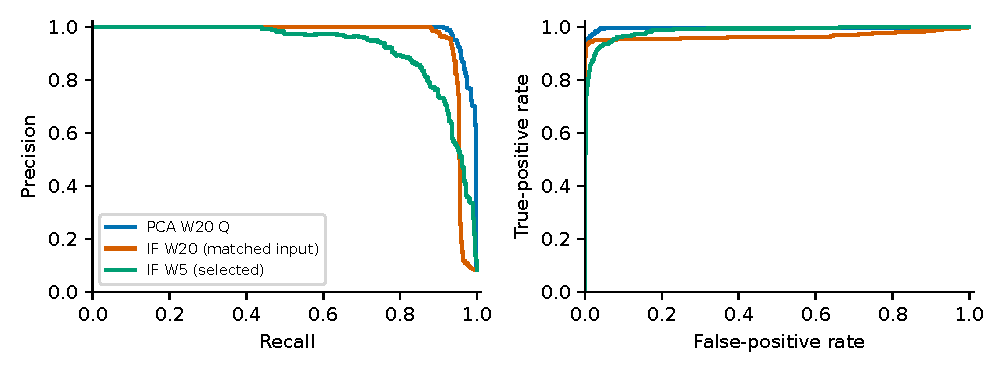
\includegraphics[width=.94\textwidth]{figures/curves.pdf}
\caption{최종 전체 행의 연속 운영 점수에 대한 PR/ROC. 이상 비율은 8.21\%다. IF W20은 입력 일치 비교, IF W5는 개발 선택 결과다. 곡선으로 최종 임계값을 재선택하지 않았다.}\label{fig:curves}
\end{figure*}

\subsection{관측 범위와 버스트 처리}
\begin{figure*}[t]
\centering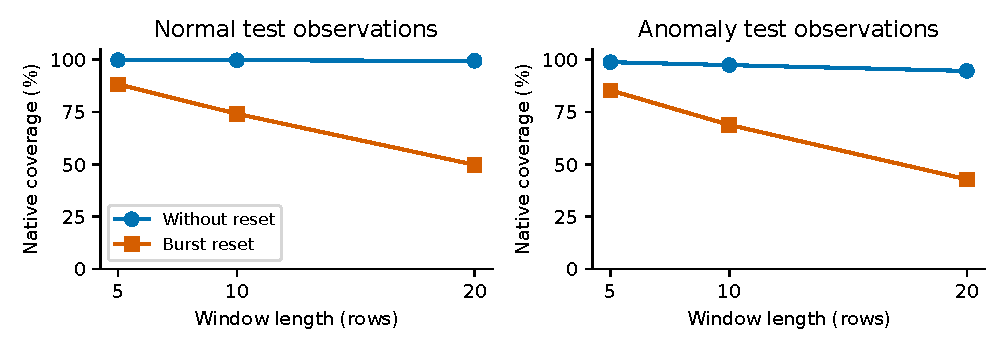
\includegraphics[width=.94\textwidth]{figures/coverage.pdf}
\caption{윈도우 모델 자체의 최종 예측 가능 비율. 정상 3,990행·이상 357행을 분모로 사용한다. 버스트 초기화 시 긴 윈도우의 관측 범위 감소가 커진다. 부족 행을 운영 평가에서 제외하지 않고 P0/I0로 보완했다.}\label{fig:coverage}
\end{figure*}

P1 W20의 자체 가용 비율은 정상 99.52\%, 이상 94.68\%지만 P2 W20은 정상 49.82\%, 이상 42.86\%다(그림~\ref{fig:coverage}). W10 P2도 정상 74.21\%, 이상 68.91\%에만 자체 점수를 낼 수 있다. 전체 운영을 완성하지 않고 이들 가용 행만 비교하면 누락된 시작부의 어려움이 숨겨진다.

선정 P1의 가용 이상은 338행이며 운영 임계값에서 323행을 탐지한다. 보완 대상 이상 19행에서는 6행만 탐지한다. 식~\ref{eq:decomp}에 따라 전체 Recall은 $(323+6)/357=92.16\%$다. 낮은 보완 성능은 가용 행의 성능만으로 운영 Recall을 예측하기 어렵다는 구체적 사례다.

같은 W10·2성분·결합 점수의 P1/P2를 동일 정상 2,961행·이상 246행에서 비교하면 초기화 후 TP는 210에서 212로 증가하고 FP는 10으로 같았다. Recall은 85.37\%에서 86.18\%, F1은 .9013에서 .9060으로 변했다. 반면 W20·2성분·$Q$의 동일 정상 1,988행·이상 153행에서는 TP가 150에서 152로 늘었으나 FP도 1에서 7로 늘어 F1이 .9868에서 .9744로 낮아졌다. 초기화의 이득은 점수와 길이에 따라 다르다.

모델별 학습 윈도우 수는 W10 P1=11,994, P2=8,948이다. 개발용에서 버스트 고려의 Recall 또는 F1 개선이 나타난 조건에 대해, 미고려 학습 마지막 행을 고려 모델 개수만큼 무작위 추출하는 보조 실험을 수행했다. W10·2성분·결합의 세 표본 반복 Recall은 모두 86.42\%이며 고려 모델의 90.12\%보다 낮았다. F1 평균도 .7985 대 .8295였다. 이 조건에서 개선이 학습 개수만의 차이로 사라지지는 않았으나 인과적 보장이나 외부 일반화의 증거는 아니다. 실제 무작위 표본 반복을 포함한 전체 적합 수는 보조 모델까지 99개다.

\subsection{$Q/T^2$ 결합의 비단조 효과}
\begin{table}[t]
\caption{선정 PCA와 같은 W20·2성분의 점수 비교. 공통 행 정상 1,988·이상 153(7.15\%)이며 각 점수는 개별 정상 보정 임계값을 사용한다.}
\label{tab:scores}\centering\small
\begin{tabular}{lrrrr}\toprule
점수 & TP & FN & FP & Recall(\%)\\\midrule
$Q$ &150&3&1&98.04\\
$T^2$ &90&63&14&58.82\\
$\max(Q/c_Q,T^2/c_T)$ &148&5&14&96.73\\\bottomrule
\end{tabular}
\end{table}

공통 행에서 $Q$만 탐지한 이상은 60개, $T^2$만 탐지한 이상은 0개였다. 결합은 $Q$ 대비 추가 이상을 탐지하지 못하고 기존 탐지 2개를 잃었으며, 기존 오경보 1개를 없애면서 새로운 정상 14개에 오경보를 냈다(표~\ref{tab:scores}). $T^2$와 결합이 항상 유리하다는 가설은 이 설정에서 지지되지 않는다. 이는 결합 점수에 재보정한 임계값이 개별 $Q$ 임계값과 다르기 때문이며, 원점수의 최대값이 크다는 사실만으로 검출 집합의 포함관계를 보장할 수 없다.

\subsection{센서 영향과 오류 조건}
센서의 비어 있지 않은 7개 조합을 원시 입력과 버스트 W10에서 비교했다. 보조 분석은 공통 정상 1,476행·이상 81행에서 이루어졌고 최종 후보 선택에 추가하지 않았다. 원시 단일 센서는 rank=1이므로 $Q$를 제외하고 $T^2$만 사용했다. 이동통계 단일 센서는 최대 5차원으로 유효한 $Q$가 가능하다. 비교의 방법 차이와 각 rank를 함께 저장했다.

W10·$Q$에서 센서 3개는 TP=77, FP=20, 진동 2개는 TP=77, FP=13, 전류만은 TP=36, FP=15였다. AI1 진동+전류는 TP=81, FP=10이었다. 이 결과는 관측 조합의 개발용 연관성을 보여주지만, 작은 선택 표본과 여러 조합 검토 때문에 특정 센서가 불필요하거나 고장 원인이라는 결론은 낼 수 없다. 이 조합을 최종 결과를 높이기 위해 다시 학습·선택하지 않았다.

주 모델의 개발 FP 8개는 모두 버스트 앞 19행의 정상 1,001행에서 발생했고, 이후 정상 985행에는 FP가 없었다. 개발용 짧은 버스트의 이상 21행 중 FN은 3개였다. 그러나 최종 짧은 버스트 이상 52행에서는 FN이 없으므로 ``짧은 구간은 항상 더 어렵다''고 일반화할 수 없다. 최종 FN 28개 중 26개는 버스트 앞 19행의 이상 204행에서 발생했고, 이 중 보완 대상 이상 19행의 FN은 13개였다. 나머지 공백을 가로지르는 윈도우에서도 13개 FN이 발생했다. 일부 윈도우는 실제 10.255초를 포괄하여 20행을 1.9초 연속 관측으로 해석할 수 없었다.

센서 절댓값과 버스트 내부 전류 변화는 정상 학습 사분위수로 구간화했다. 개발 정상의 전류 변화 최상위 구간 399행 중 FP는 2개, 두 번째 구간 475행 중 FP는 4개였다. 변화량 증가에 따른 단조로운 오경보 증가는 관찰되지 않았다. 실제 부하·공정 상태가 없으므로 이 구간은 관측값 조건이며 물리적 운전조건을 대신하지 않는다.

$Q=\sum_f(z_f-\hat z_f)^2$를 특징별로 분해하고 같은 센서의 다섯 항을 묶었다. FP/FN 파일에는 원래 행, 시각, 센서, 버스트 위치, 윈도우 시작/종료, 실제 경과시간, $Q/T^2/QT$, 적용 임계값과 보완 경로를 저장했다. 기여는 점수의 대수적 구성이지 인과적 고장 원인이 아니며 주성분 계수만으로 원인 센서를 확정하지 않는다.

\subsection{후처리, 확률 보정, 시간 해석}
연속 2회 및 최근 3회 중 2회 경보를 개발 자료에서 비교하고 파일·분할·버스트마다 상태를 초기화했다. 미래 경보를 과거로 소급하지 않는다. 개발 선택은 후처리 없음으로 고정했다. 최종 연속 2회 정책은 FP를 1에서 0으로 줄였지만 FN을 28에서 46으로 늘렸다. 최근 3회 중 2회는 FN=41, FP=0이었다. 두 정책 모두 길이 20 미만의 이상 52행에서 기본 정책에 없던 FN 5개를 만들었다.

\begin{table}[t]
\caption{선정 모델의 최종 후처리 비교. 정상 3,990·이상 357행. 원시 점수와 임계값은 고정한다.}
\label{tab:post}\centering\small\setlength{\tabcolsep}{4pt}
\begin{tabular}{lrrrrr}\toprule
정책 & FN & FP & Recall(\%) & F1 & F2\\\midrule
없음 &28&1&92.16&.9578&.9357\\
연속 2회 &46&0&87.11&.9311&.8942\\
최근 3회 중 2회 &41&0&88.52&.9391&.9060\\\bottomrule
\end{tabular}
\end{table}

실제 고장 시작이나 정상→이상 전환 시각이 없으므로 계산 가능한 시간은 \emph{관측 버스트 시작부터 첫 경보까지}다. 이상 13개 관측 버스트에는 모든 정책에서 최소 한 번 경보가 있었지만, 이를 독립 고장 13건을 모두 탐지했다고 해석하거나 전체 행을 정답 처리하지 않는다. 첫 경보 시간의 중앙값은 기본 0.0초, 두 후처리 0.1초다. 미경보 구간을 숨기지 않는 전체 목록을 제공하고, 0초라는 값은 고장 전 예측의 증거가 아니다. 윈도우 준비시간과 CPU 계산시간을 별도로 저장한다.

추가 확률 실험에서는 보정 정상 2,011행과 이상 132행의 라벨로 sigmoid를 적합했다. 입력은 운영 점수의 $\log(1+S)$를 보정 자료의 평균·표준편차로 변환한 값이며, 비음수 기울기와 $10^{-4}$ 정규화를 적용했다. 선택 자료에서 Brier=.001984, log loss=.01610, 최종에서는 .008123과 .03515였다. 보정 이상 비율 상수 예측의 최종 값은 각각 .07580, .28725다. 신뢰도 bin별 개수를 함께 제공하며, Brier 한 값으로 완벽한 확률 보정을 주장하지 않는다. 보정 이상이 4버스트뿐이고 이상 비율도 보정 6.16\%에서 최종 8.21\%로 달라 현장 사전확률 변화에 대한 검증이 필요하다. 이 추가 지도 보정은 주 경보 임계값 선택을 대체하지 않는다.

\section{논의와 한계}
\paragraph{비교의 범위.}
단일 사례에서 PCA가 IF보다 우수한 조건을 관찰했지만 전반적인 모델 우월성을 주장할 수 없다. 특히 개발용 최적 IF W5는 최종의 동일 입력 IF W20보다 낮은 Recall을 보였다. 모델 선택 자료가 이상 111행·4버스트에 불과해 날짜 내 변화에도 선택 순위가 불안정할 수 있다. F1 대안은 개발에서 같은 PCA의 목표 0.5\% 임계값을 선택했으나 최종 TP=325, FP=0, F1=.9531로 주 임계값 F1=.9578보다 낮았다. 최종 점수를 보고 이를 바꾸지 않았다.

\paragraph{날짜와 사건의 교란.}
모든 정상과 이상이 서로 다른 날짜에 존재하므로 센서 차이가 건강 상태인지 날짜·부하 차이인지 식별할 수 없다. 시간 분할은 행 누수를 막지만 이 교란을 해결하지 못한다. 버스트는 데이터 취득 구간일 뿐 독립 고장 사건이 아니다. 행별 iid 신뢰구간이나 의미 없는 유의확률을 제시하지 않았다. 버스트 재표집도 날짜 단위 독립 고장 일반화를 보장하지 않으며 본 연구에서는 수행하지 않았다.

\paragraph{현장 해석.}
점수 배수는 점검 우선순위를 위한 관측 증거로 활용할 수 있으나 압력 불안정, 불량 감소, 비가동 감소의 직접 검증은 아니다. 라벨 비율과 날짜가 달라지면 Precision과 보정 확률이 달라진다. 경보 후처리가 드문 FP를 없애더라도 더 많은 이상 행을 놓칠 수 있다. 그러므로 오경보 감소만을 현장 효용으로 보고하지 않는다.

\paragraph{ICML 수준으로 확장하기 위한 미완료 검증.}
현재 연구는 기존 방법의 정밀한 적용·평가 사례다. 독립 날짜·설비·실제 고장 사건의 외부 자료, 사전 등록된 새 holdout, 동일 예산의 추가 기준 모델, 관측 공백 효과의 여러 데이터셋 반복이 확보되어야 넓은 주장과 강한 학술적 기여를 검토할 수 있다. 추가 자료 없이 형식만 바꾸어 그 수준을 충족했다고 주장하지 않는다. 이미 확인한 최종 자료는 새 선택용 holdout으로 재사용하지 않는다.

\section{결론}
시간 공백 처리, 예측 가능 범위, 임계값 보정과 보완 정책을 명시한 PCA/IF 비교를 수행했다. 선정 P1 W20 $Q$는 최종 이상 329/357행을 탐지하고 정상 1/3,990행에 오경보를 냈다. 동일 입력 IF와의 차이는 탐지 9행과 오경보 5행이며, 버스트 초기화·$Q/T^2$ 결합·경보 지속 조건의 효과는 조건부였다. 공통 행 성능과 전체 운영 성능을 함께 기록하는 것이 중요하며, 본 결과는 실제 고장 전 조기예측이나 여러 설비의 일반화 검증을 대체하지 않는다.

\section*{재현성과 연구 영향}
원본 CSV 두 개, 고정 행 목록, 모든 후보 결과·seed, 모델 객체, 코드, 실험 및 논문 작성용 에이전트 명령문을 첨부 패키지로 제공한다. 데이터의 공식 배포처 식별자와 재배포 조건은 사용자 제공 자료에서 확정되지 않았으므로 해당 정보를 데이터 카드에 미확인으로 기록했다. 본 패키지는 사용자에게 전달하는 연구 작업물이며 공개 배포나 학회 제출을 수행한 것은 아니다. 저자·소속·이해관계는 연구 책임자가 확인할 항목으로 남겼다. AI 에이전트는 코드 실행·검사·원고 작성에 사용되었고, 수치의 근거 파일과 실행 문제를 공개한다. 현장 경보를 자동 정지나 고장 확정으로 오용할 경우 생산·점검 비용을 발생시킬 수 있으므로 본 연구의 관측 기반 판정을 실제 고장 판정과 구분한다.

\bibliography{references}
\bibliographystyle{icml2026}
\clearpage
\appendix
\onecolumn
\section{실험 설계와 구현 세부}
\begin{table}[h]\centering\small
\begin{tabularx}{\textwidth}{lX}\toprule
항목 & 고정 정의\\\midrule
입력·전처리 & 센서 3개 또는 시간영역 15특징. 부호 유지, 정상 학습 StandardScaler. FFT·값 클리핑 없음.\\
버스트 & 중복 제거 후 간격 $>0.5$초. 파일·분할·train\_role 경계도 넘지 않음.\\
PCA & full SVD, whiten=False. P0: 1/2성분; P1/P2: 2/3/5/8성분. 유효 rank보다 적은 성분의 $Q$만 허용.\\
IF & 300 trees, max\_samples=256, contamination=auto, n\_jobs=2, seed 42/43/44, $-\mathrm{score\_samples}$.\\
점수 & $Q,T^2,\max(Q/c_Q,T^2/c_T)$. 정상 보정 95백분위수 참조. 참조 $\leq10^{-12}$ 제외.\\
임계값 & 목표 FPR .005/.01/.02/.05, quantile higher, score$>$threshold, 동점 정상.\\
선택 & 전체 행 운영, 선택 FPR$\leq.01$ 제약 후 Recall/F1/AP/실행시간 순. 적격 없음 명시.\\
보완 & PCA는 공통 P0; IF는 seed별 I0. 각 점수를 자기 정상 보정 95백분위수로 나눈 뒤 연결·재보정.\\
후처리 & 없음, 연속 2회, 최근 3회 중 2회. 버스트마다 초기화, 과거 소급 없음.\\
확률 & 보정 라벨을 쓰는 비음수 기울기 sigmoid, log1p 점수 표준화, 정규화 $10^{-4}$.\\
분모 예외 & 양성 예측 없음의 Precision=0; F1/F2 미정의=0. 클래스 없음의 해당 비율 및 순위 지표는 결측.\\\bottomrule
\end{tabularx}
\end{table}

\paragraph{환경과 실제 검사.}
실제 모델 실험은 전용 Colab CPU 세션에서 Python 3.13.15, NumPy 2.5.3, pandas 3.0.6, SciPy 1.18.1, scikit-learn 1.9.1, matplotlib 3.11.2로 수행했다. CPU 스레드는 2개로 제한했다. 로컬 전용 환경은 Python 3.14.4와 동일한 잠금 라이브러리를 사용했다. 다른 환경의 시간을 직접 순위 비교하지 않는다. 99개 저장 모델의 scaler 평균을 실제 정상 학습 입력에서 재계산해 확인했고, 입력 allowlist·시간 경계·유효 rank·IF 점수 방향·미래값 변경 불변성·seed 공개·공통 분모를 검사했다. 다운로드한 761개 원격 파일의 해시를 검증했으며, 라벨 없는 로컬 입력으로 최종 4,347행의 경보 판정이 모두 일치했다. 점수 차이는 최대 $2.85\times10^{-14}$ 이하였다. 사용한 전용 Colab 세션만 종료했다.

\paragraph{오류 수정 이력.}
전용 환경의 ensurepip 실패는 해당 환경을 pip 없이 만든 뒤 설치 도구가 그 환경을 직접 대상으로 사용하게 하여 해결했다. Colab의 notebook backend 충돌은 matplotlib import 전 Agg 설정으로 해결했다. 개발용 주 모델과 F1 대안의 이름이 같아 오류 파일명이 겹친 저장 문제는 목표 FPR를 파일명에 넣어 수정했다. 원래 파일도 보존하되 \code{target0p01}/\code{target0p005} 파일을 공식 진단으로 사용한다. 검사 결과의 NumPy bool 직렬화 문제도 수정했다. 최종 평가로 모델을 재선택하거나 최종 성능을 높이기 위한 재실행은 하지 않았다.

\section{수치 근거와 파일 대응}
\begin{table}[h]\centering\small
\begin{tabularx}{\textwidth}{lX}\toprule
주장·분석 & 패키지 내 근거(결과 기준 디렉터리: \code{results/\allowbreak pca\_\allowbreak 20261003\_\allowbreak cpu/\allowbreak })\\\midrule
원본·중복·간격·분할 & \code{manifests/\allowbreak audit.json}, \code{manifests/\allowbreak clean\_\allowbreak rows.csv}, \code{manifests/\allowbreak configs/\allowbreak first\_\allowbreak experiment/\allowbreak }\\
선택과 최종 고정 & \code{selection\_\allowbreak lock.json}, \code{final\_\allowbreak summary.json}, \code{manifests/\allowbreak final\_\allowbreak evaluation\_\allowbreak started.json}\\
표 2 및 공통 행 비교 & \code{tables/\allowbreak metrics\_\allowbreak with\_\allowbreak counts\_\allowbreak test.csv}, \code{tables/\allowbreak best\_\allowbreak by\_\allowbreak family\_\allowbreak test.csv}\\
버스트·관측 범위·표본 수 & \code{tables/\allowbreak burst\_\allowbreak pairs\_\allowbreak test.csv}, \code{tables/\allowbreak coverage.csv}, \code{tables/\allowbreak matched\_\allowbreak training\_\allowbreak count\_\allowbreak selection.csv}\\
$Q/T^2$ 및 센서 조합 & \code{tables/\allowbreak score\_\allowbreak complements\_\allowbreak test.csv}, \code{tables/\allowbreak sensor\_\allowbreak combinations\_\allowbreak selection.csv}\\
행별 오류·기여·경로 & \code{predictions/\allowbreak errors\_\allowbreak *\_\allowbreak target0p01\_\allowbreak test.csv}, \code{predictions/\allowbreak all\_\allowbreak candidate\_\allowbreak errors\_\allowbreak test.csv.gz}, \code{predictions/\allowbreak all\_\allowbreak routes\_\allowbreak test.csv.gz}\\
후처리와 시간 & \code{tables/\allowbreak postprocess\_\allowbreak test.csv}, \code{tables/\allowbreak postprocess\_\allowbreak conditions\_\allowbreak test.csv}, \code{tables/\allowbreak postprocess\_\allowbreak paired\_\allowbreak delays\_\allowbreak test.csv}\\
확률과 신뢰도 & \code{tables/\allowbreak probability\_\allowbreak test.csv}, \code{tables/\allowbreak reliability\_\allowbreak test.csv}, \code{models/\allowbreak sigmoid.json}\\
재현 검사 & \code{manifests/\allowbreak development\_\allowbreak validation.json}, \code{manifests/\allowbreak final\_\allowbreak artifact\_\allowbreak validation.json}\\\bottomrule
\end{tabularx}
\end{table}

\paragraph{데이터 식별.}
원본 정상 CSV SHA-256은 \texttt{\scriptsize f2d61cb3b3108f49a3305d2966b3a31f26942ac8af8ffc9eb531b432b945b0a7}, 이상 CSV는 \texttt{\scriptsize 9fad8c238e63dba3257d8be32a32362548955c772171a95c0d2af61b0435ed2e}이다. 고정 행 목록의 SHA-256은 \texttt{\scriptsize 9372ae29ed7d3104a0d88c20b961a2aef034ff7b96b5735aac5f2c0c50de16c2}다. 원본은 수정하지 않았다. 파일명·원래 데이터 행 번호·CSV 줄 번호를 보존하여 오류를 원자료까지 추적할 수 있다.

\section{재실행과 에이전트 명령문}
압축을 풀고 루트 디렉터리에서 \code{bash RUN\_\allowbreak EXPERIMENT.sh}를 실행한다. 새 전용 가상환경 및 새 결과 폴더를 사용하며 기존 결과를 덮어쓰지 않는다. 모델을 재학습하지 않는 패키지 검사는 \code{bash VERIFY\_\allowbreak PACKAGE.sh}, 논문 재편집은 \code{bash BUILD\_\allowbreak PAPER.sh}로 실행한다. 라이브러리와 TeX 의존성의 최초 설치에는 네트워크가 필요할 수 있다. 저장 모델은 Python/scikit-learn 버전 의존 객체이므로 잠금 환경을 사용한다.

실험용 전체 지시는 \code{agent/\allowbreak EXPERIMENT\_\allowbreak AGENT\_\allowbreak PROMPT\_\allowbreak KO.txt}, 논문 작성·확장용 지시는 \code{agent/\allowbreak PAPER\_\allowbreak AGENT\_\allowbreak PROMPT\_\allowbreak KO.txt}에 포함한다. 이 문서는 사용자의 조건을 실행 가능하게 정리한 명령문이며 대화 원문 전사라고 주장하지 않는다. 명령문에는 원자료·다른 작업 영역 보호, 고정 분할, 정상 fit, 개발 라벨 사용 공개, 106개 점수 구성의 전체 공개, 최종 데이터 재튜닝 금지, 오류 복구 기록과 산출물 검증을 포함한다. 논문 부록의 짧은 재현 명령과 파일 경로만으로도 전체 코드·데이터·결과에 접근할 수 있다.

\section{평가 항목 대응과 후속 연구 계획}
\begin{table}[h]\centering\small
\begin{tabularx}{\textwidth}{lXX}\toprule
평가 항목 & 수행 및 실제 근거 & 한계\\\midrule
데이터 이해·진단 & 해시·중복 1행·598/20개 공백·시간순 분할 공개 & 단위·부하·공식 데이터 배포 식별자 미확인\\
모델 개발·비교 & PCA/IF, 같은 행과 전체 행 비교; TP329/FN28/FP1 & 단일 날짜쌍, 전체 비지도 절차 아님\\
영향요인·오류 & 7센서 조합, 조건별 정상/이상 분모, 특징별 $Q$ & 기여는 원인 인과성 아님\\
현장 활용 & 부족 행 보완, 후처리, 실제 관측 첫 경보 시간 & 실제 고장 시작·압력·품질·비가동 검증 없음\\
차별성 & 관측 범위와 보완 분리, 점수 결합의 부정적 결과 공개 & 새 알고리즘 발명 주장 없음\\
재현성 & 원본·고정 설정·모든 seed·모델·코드·명령문·해시 & CPU·버전별 시간 차이; 배포 권리 추가 확인 필요\\\bottomrule
\end{tabularx}
\end{table}

향후 검증은 새 자료 확보 후 별도 프로토콜로 수행해야 한다. (1) 같은 날짜의 정상/이상과 여러 날짜·설비를 포함해 교란을 줄이고, (2) 정상→이상 전환과 정비 시점을 수집하여 실제 조기탐지 지표를 정의하고, (3) 새 날짜/설비 holdout을 먼저 잠그고, (4) 동일 관측·임계값 예산의 기준 모델을 사전에 정한다. 표본 수에 기반한 검정력 분석과 날짜/설비/고장 사건 단위 불확실성 추정은 그때 수행할 일이며 현재 실행한 결과로 표시하지 않는다. 기존 최종 평가 자료를 다시 선택용으로 사용하는 계획은 포함하지 않는다.
\end{document}
